\documentclass{article}


%pacchetti extra da scaricare dblfloatfix, fancyhdr
\usepackage{fancyhdr}%creazione header-footer
\usepackage{graphicx} %serve per inserire immagini
%\usepackage{dblfloatfix} %serve per posizionare gli elementi dove si vuole
\usepackage[hidelinks]{hyperref} %serve per i link
\usepackage{tikz}
% \usepackage{tgadventor} % font
\usepackage[useregional=numeric,showseconds=true,showzone=false]{datetime2}
\usepackage{caption}
\usepackage{geometry}
\usepackage{setspace}
\usepackage{eurosym}
\usepackage[italian]{babel}
\usepackage[hidelinks]{hyperref}
\usepackage{tabularx}
\usepackage{longtable}
\usepackage{float}
\usepackage{graphicx}
% Margini della pagina
\geometry{a4paper, margin=1in}

% Intestazione personalizzata
\pagestyle{fancy}
\fancyhf{}
\fancyhead[L]{Code7Crusaders - Software Development Team}
\fancyhead[R]{\thepage}

% Spaziatura delle righe
\setstretch{1.2}

\begin{document}

\begin{titlepage} 

    \AddToHookNext{shipout/background}{
    \begin{tikzpicture}[remember picture,overlay]
    \node at (current page.center) {
    \includegraphics{../../../img/background.png}
    };
    \end{tikzpicture}
    }

    \centering
    \vspace*{2cm}
    
    \includegraphics[width=0.3\textwidth]{../../../img/logo/7Crusaders_logo.png} % Aggiungi il logo qui
    \vspace{1cm}
    
    {\Huge \textbf{Code7Crusaders}}\\
    \vspace{0.5cm}
    {\Large Software Development Team}\\
    \vspace{2cm}
    
    \large \textbf{Manuale Utente}
    \vspace{3.9cm}

    \textbf{Membri del Team:}\\
    Enrico Cotti Cottini, Gabriele Di Pietro, Tommaso Diviesti \\
    Francesco Lapenna, Matthew Pan, Eddy Pinarello, Filippo Rizzolo \\
    \vspace{0.5cm}
    
    \vspace{1cm}
\end{titlepage}



\newpage
%------------------------Versioni
\begin{table}[h]
    \centering
    \renewcommand{\arraystretch}{1.2}
    \setlength{\tabcolsep}{5pt}
    \begin{tabular}{|c|c|c|c|m{0.35\textwidth}|}
        \hline
        \textbf{Ver} & \textbf{Data} & \textbf{Redattore} & \textbf{Verificatore} & \textbf{Descrizione} \\
        \hline
        0.2 & 29/03/2025 & Filippo Rizzolo & & Stesura \\
        0.1 & 1/03/2025 & Eddy Pinarello & Filippo Rizzolo & Prima stesura del documento \\
        \hline
    \end{tabular}
\end{table}

%----------------

\newpage
\tableofcontents
\listoftables
\listoffigures

\newpage

\section{Introduzione}

\subsection{Scopo del documento}
Questo documento mira a offrire una panoramica dettagliata del prodotto, 
delineando i bisogni degli utenti in base alle diverse categorie individuate durante 
l'analisi del capitolato e gli incontri con il committente.
L'obiettivo è identificare chiaramente tutti i requisiti e gli attori coinvolti
nel sistema software, garantendo una descrizione accurata delle componenti del programma
e una visione strutturata delle attività da svolgere. 

I casi d’uso seguono una struttura logica ben definita e vengono descritti 
con precisione secondo i seguenti punti chiave:

\begin{itemize}
    \item \textbf{Descrizione}: Titolo del caso d’uso accompagnato da un breve commento esplicativo;
    \item \textbf{Attori coinvolti}: Soggetti che interagiscono con il sistema;
    \item \textbf{Precondizioni}: Stato del sistema prima dell’avvio del caso d’uso;
    \item \textbf{Postcondizioni}: Stato del sistema al termine dello scenario del caso d’uso;
    \item \textbf{Scenario principale}: Sequenza di azioni che collega le precondizioni ai risultati, descrivendo il flusso principale dello scenario.
\end{itemize}

\subsection{Scopo del prodotto}
Il prodotto descritto in questo documento ha come obiettivo...

\subsection{Glossario}
Nel seguente glossario sono definiti i termini tecnici utilizzati nel documento...

\subsection{Maturità e miglioramenti}
Il prodotto ha raggiunto un livello di maturità tale da...

\subsection{Riferimenti}

\subsubsection{Riferimenti normativi}
I seguenti riferimenti normativi sono stati utilizzati...

\subsubsection{Riferimenti informativi}
I seguenti riferimenti informativi sono stati utilizzati...


\newpage

\section{Requisiti}
Per garantire un corretto funzionamento del prodotto è necessario rispettare alcuni requisiti minimi. Questi requisiti sono stati suddivisi in due categorie: hardware e software. La prima categoria riguarda le specifiche tecniche del computer o del dispositivo su cui verrà eseguito il programma, mentre la seconda si riferisce ai programmi e alle librerie necessarie per il corretto funzionamento dell'assistente virtuale.
I requisiti minimi sono stati definiti in modo da garantire prestazioni ottimali e un'esperienza utente fluida. È importante notare che, sebbene il programma possa funzionare su dispositivi con specifiche inferiori, potrebbero verificarsi rallentamenti o malfunzionamenti. Pertanto, si consiglia di utilizzare un dispositivo che soddisfi o superi i requisiti minimi indicati di seguito.

\subsection{Requisiti hardware}
Poiché l'assistente virtuale è un'applicazione web, non sono richieste specifiche hardware particolari. Tuttavia, per garantire prestazioni ottimali, si consiglia di utilizzare un computer con le seguenti caratteristiche minime:
\begin{itemize}
    \item \textbf{Processore:} Intel Core i5 o equivalente
    \item \textbf{RAM:} 8 GB
    \item \textbf{Spazio su disco:} 10 GB di spazio libero
    \item \textbf{Connessione a Internet:} necessaria per l'accesso ai servizi online e per il download delle librerie necessarie
\end{itemize}

\subsection{Requisiti software}
Poichè l'assistente virtuale è un'applicazione web, è necessario possedere un browser aggiornato. Si consiglia di utilizzare uno dei seguenti browser:
\begin{itemize}
    \item \textbf{Google Chrome} (versione 90 o superiore)
    \item \textbf{Mozilla Firefox} (versione 85 o superiore)
    \item \textbf{Microsoft Edge} (versione 90 o superiore)
    \item \textbf{Safari} (versione 14 o superiore)
    \item \textbf{Arc} (versione 1.0 o superiore)
\end{itemize}

\newpage

\section{Istruzioni all'uso}

\subsection{Landing page}
All'avvio del prodotto verrà visualizzata la landing page, che presenta il logo dell'assistente virtuale e un messaggio di benvenuto. In questa fase, l'utente può scegliere di accedere al sistema.
\begin{figure}[h!]
    \centering
    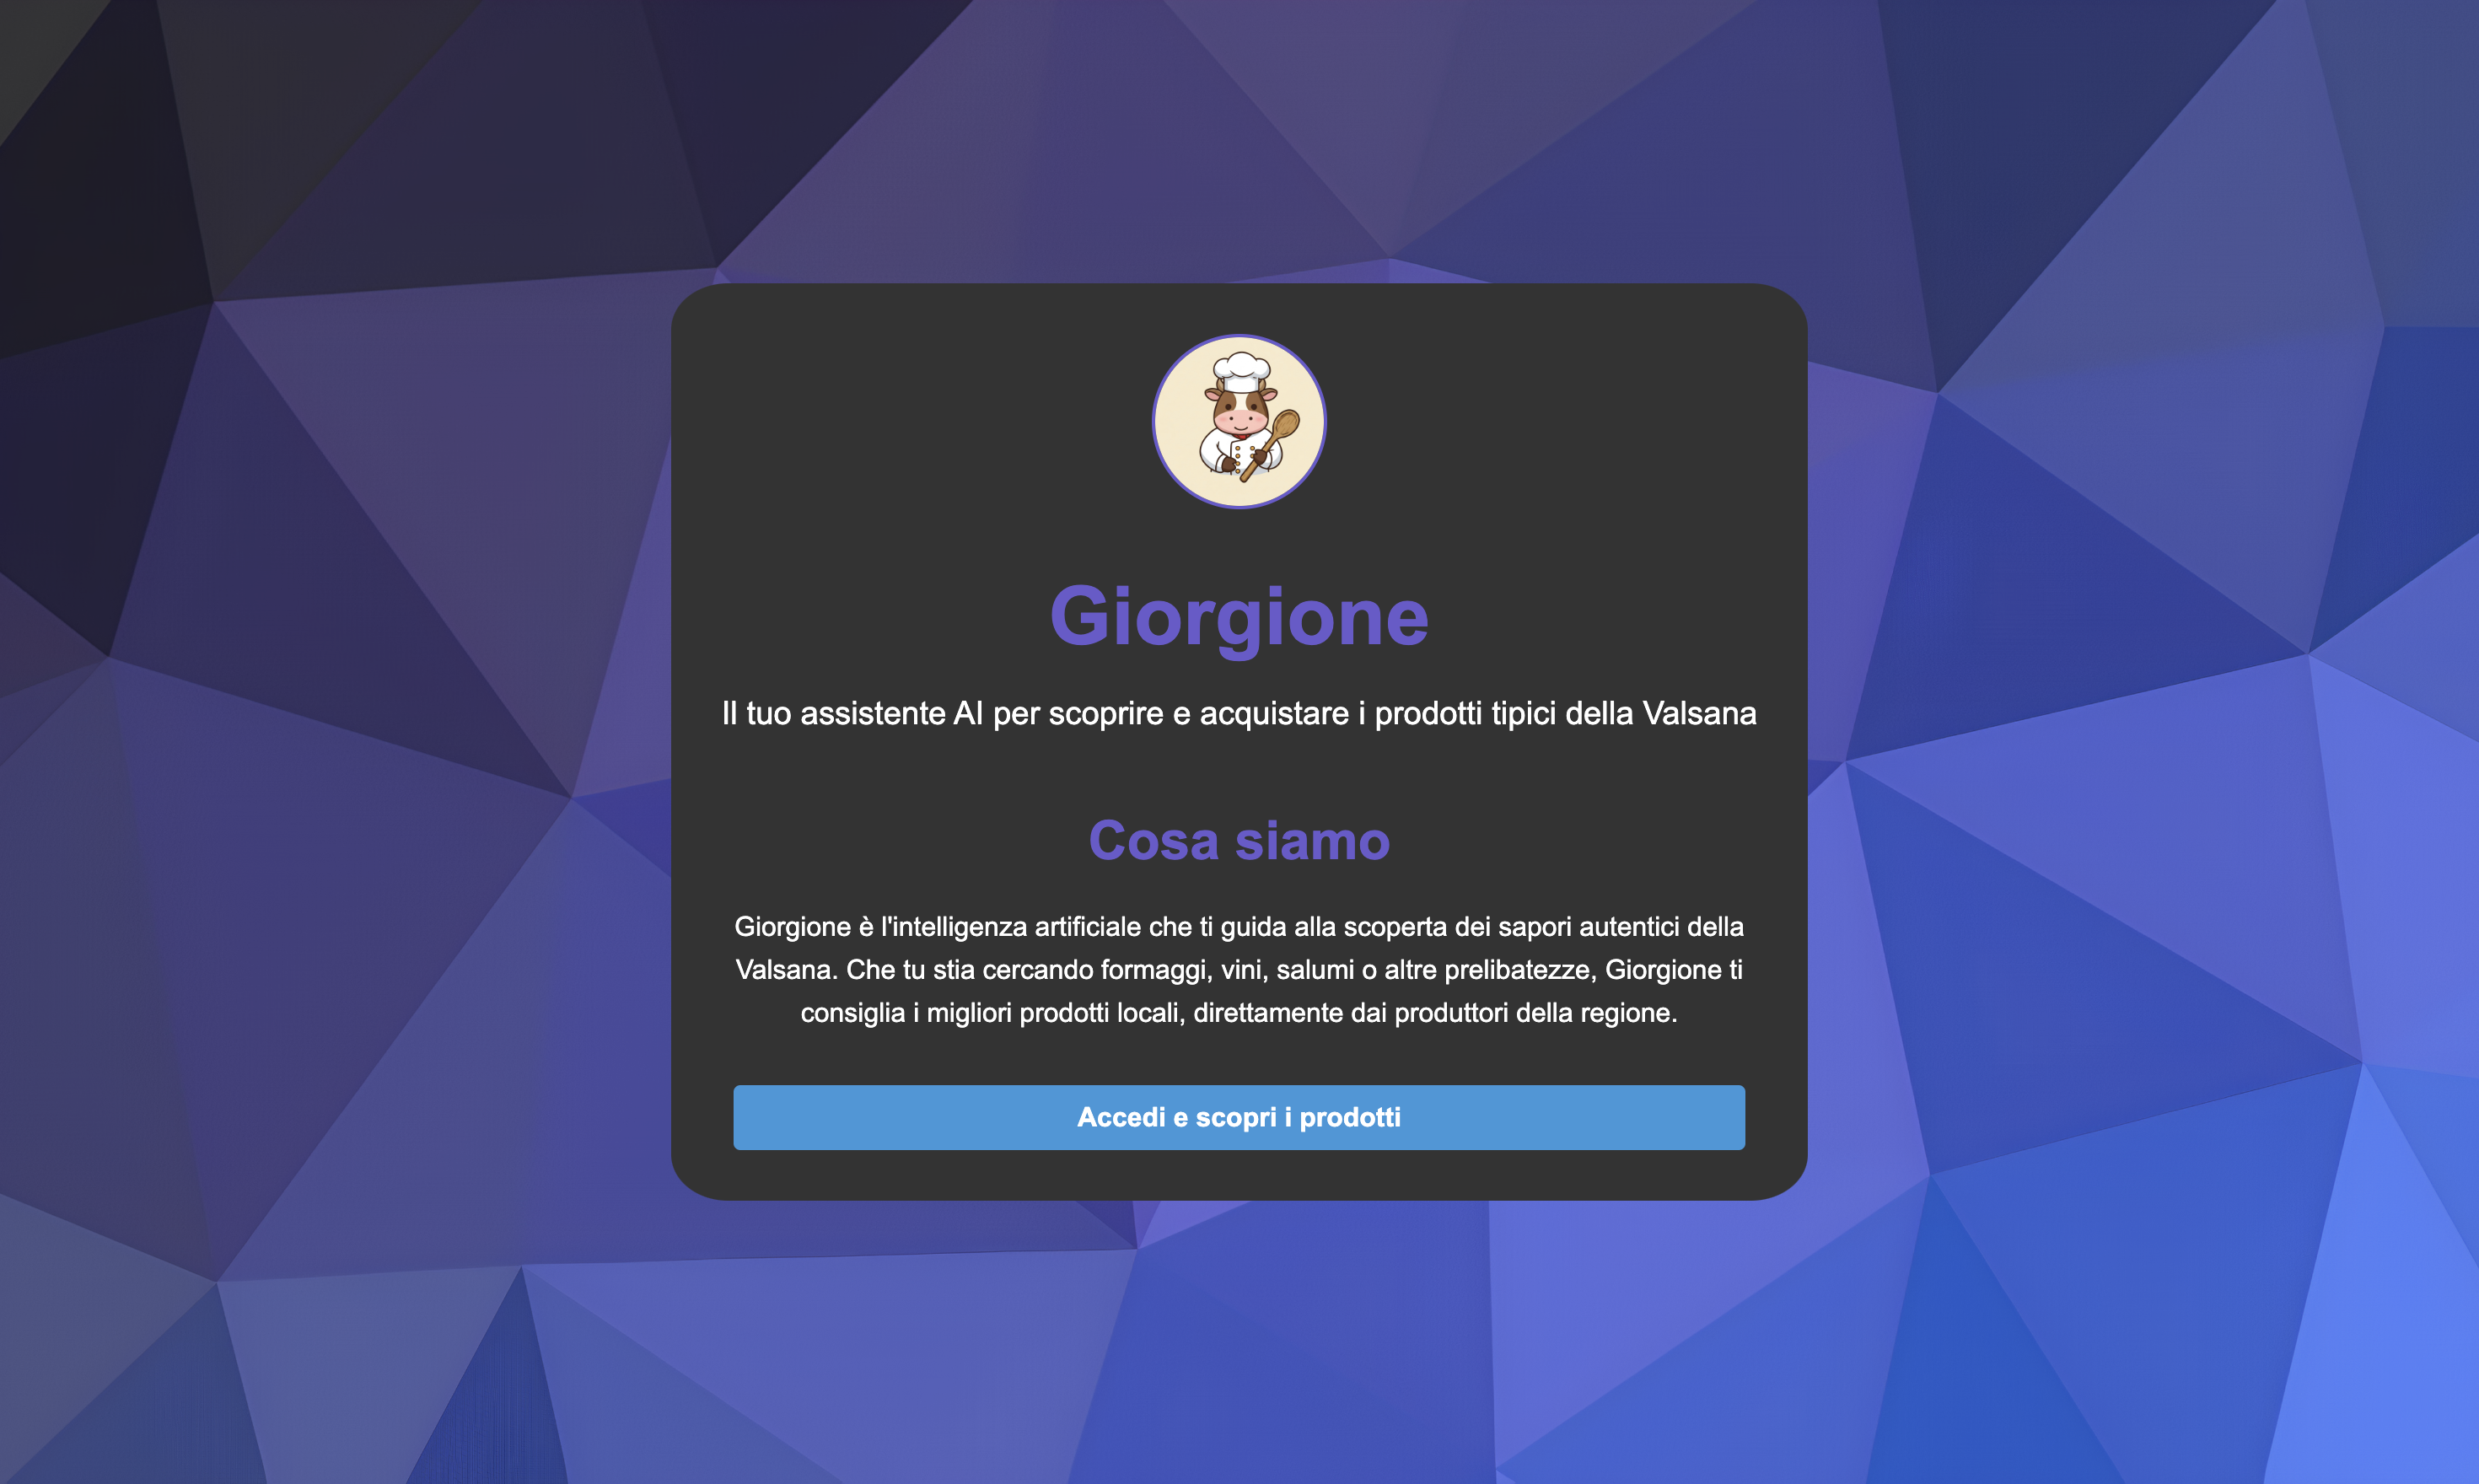
\includegraphics[width=0.8\textwidth]{./img/landingPage.png}
    \caption{Schermata della landing page}
\end{figure}

\subsection{Pagina di Accesso}
Cliccando sul bottone blu si passerà direttamente alla pagina di accesso, dove l'utente dovrà inserire le proprie credenziali (\textit{username} e \textit{password}) per autenticarsi.
\begin{figure}[h!]
    \centering
    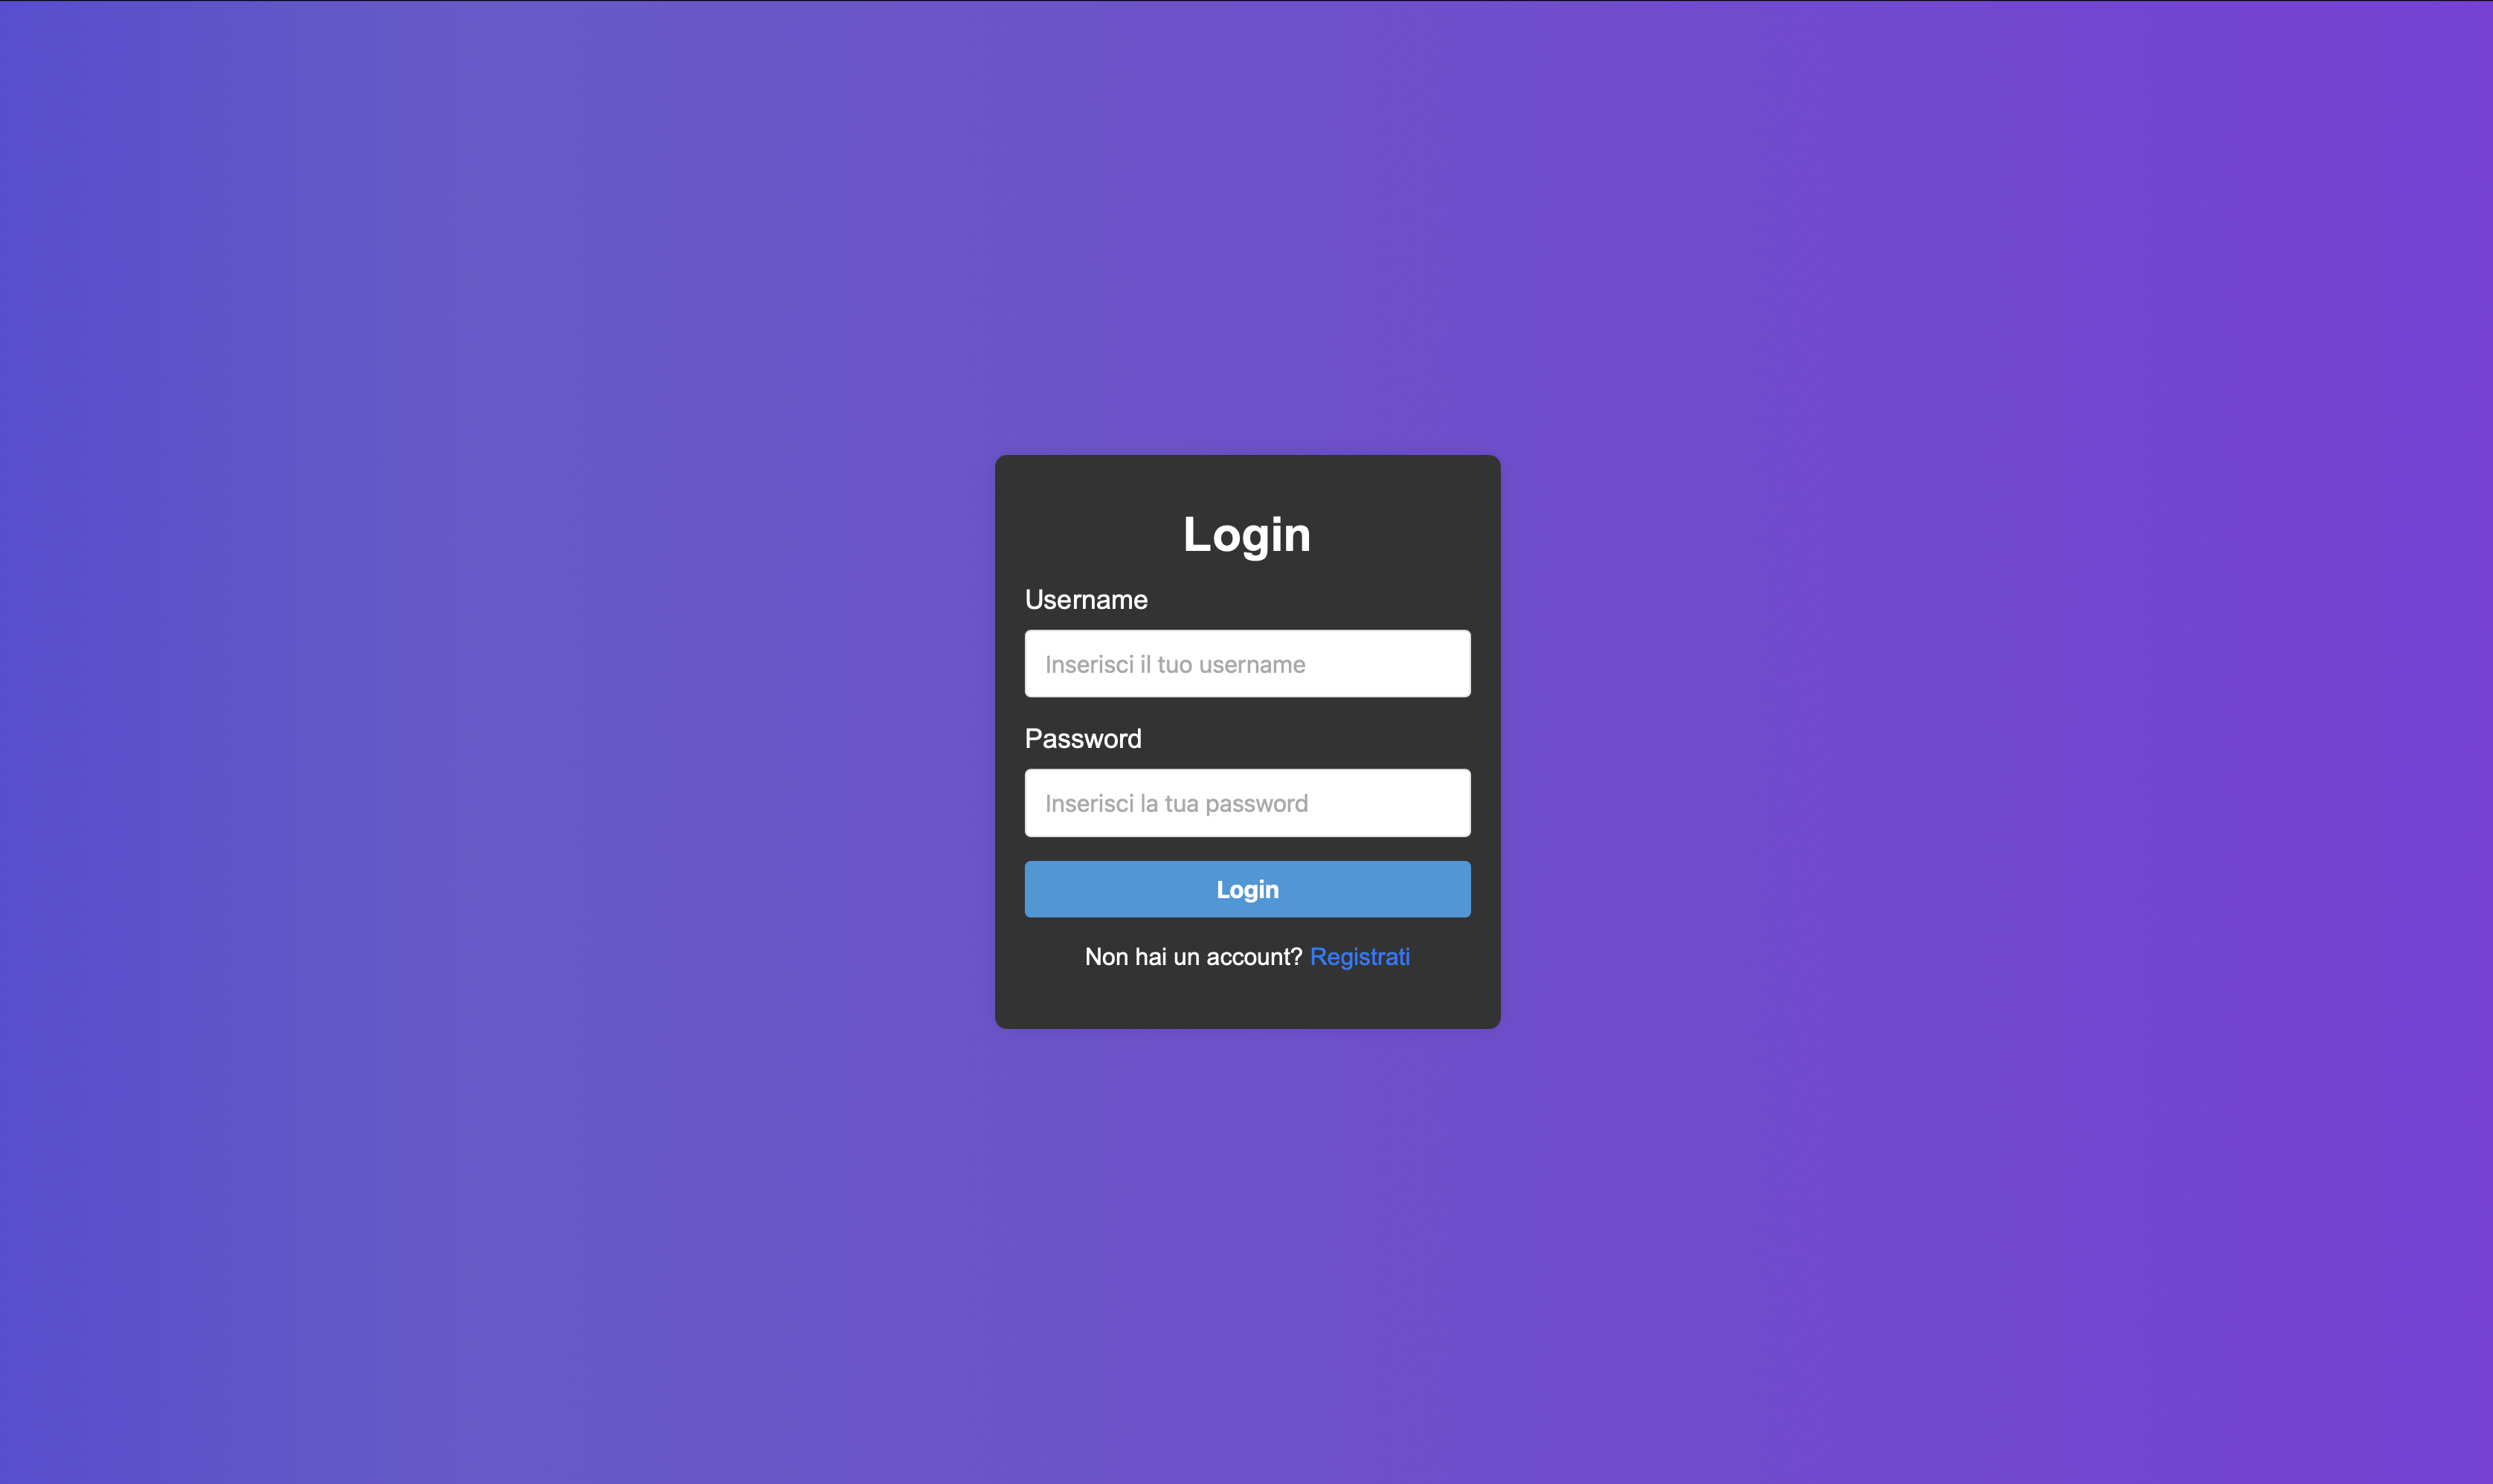
\includegraphics[width=0.8\textwidth]{./img/paginaAccesso.png}
    \caption{Schermata della pagina di accesso}
\end{figure}

\subsection{Pagina di Registrazione}
Nel caso in cui non si possieda un account, è possibile registrarsi dalla pagina di registrazione cliccando sul link presente nella pagina di autenticazione.
Qui l'utente dovrà inserire i campi obbligatori \{ \textit{username; password; email; nome; cognome} \} e volendo opzionalmente può inserire il numero di telefono.
\begin{figure}[h!]
    \centering
    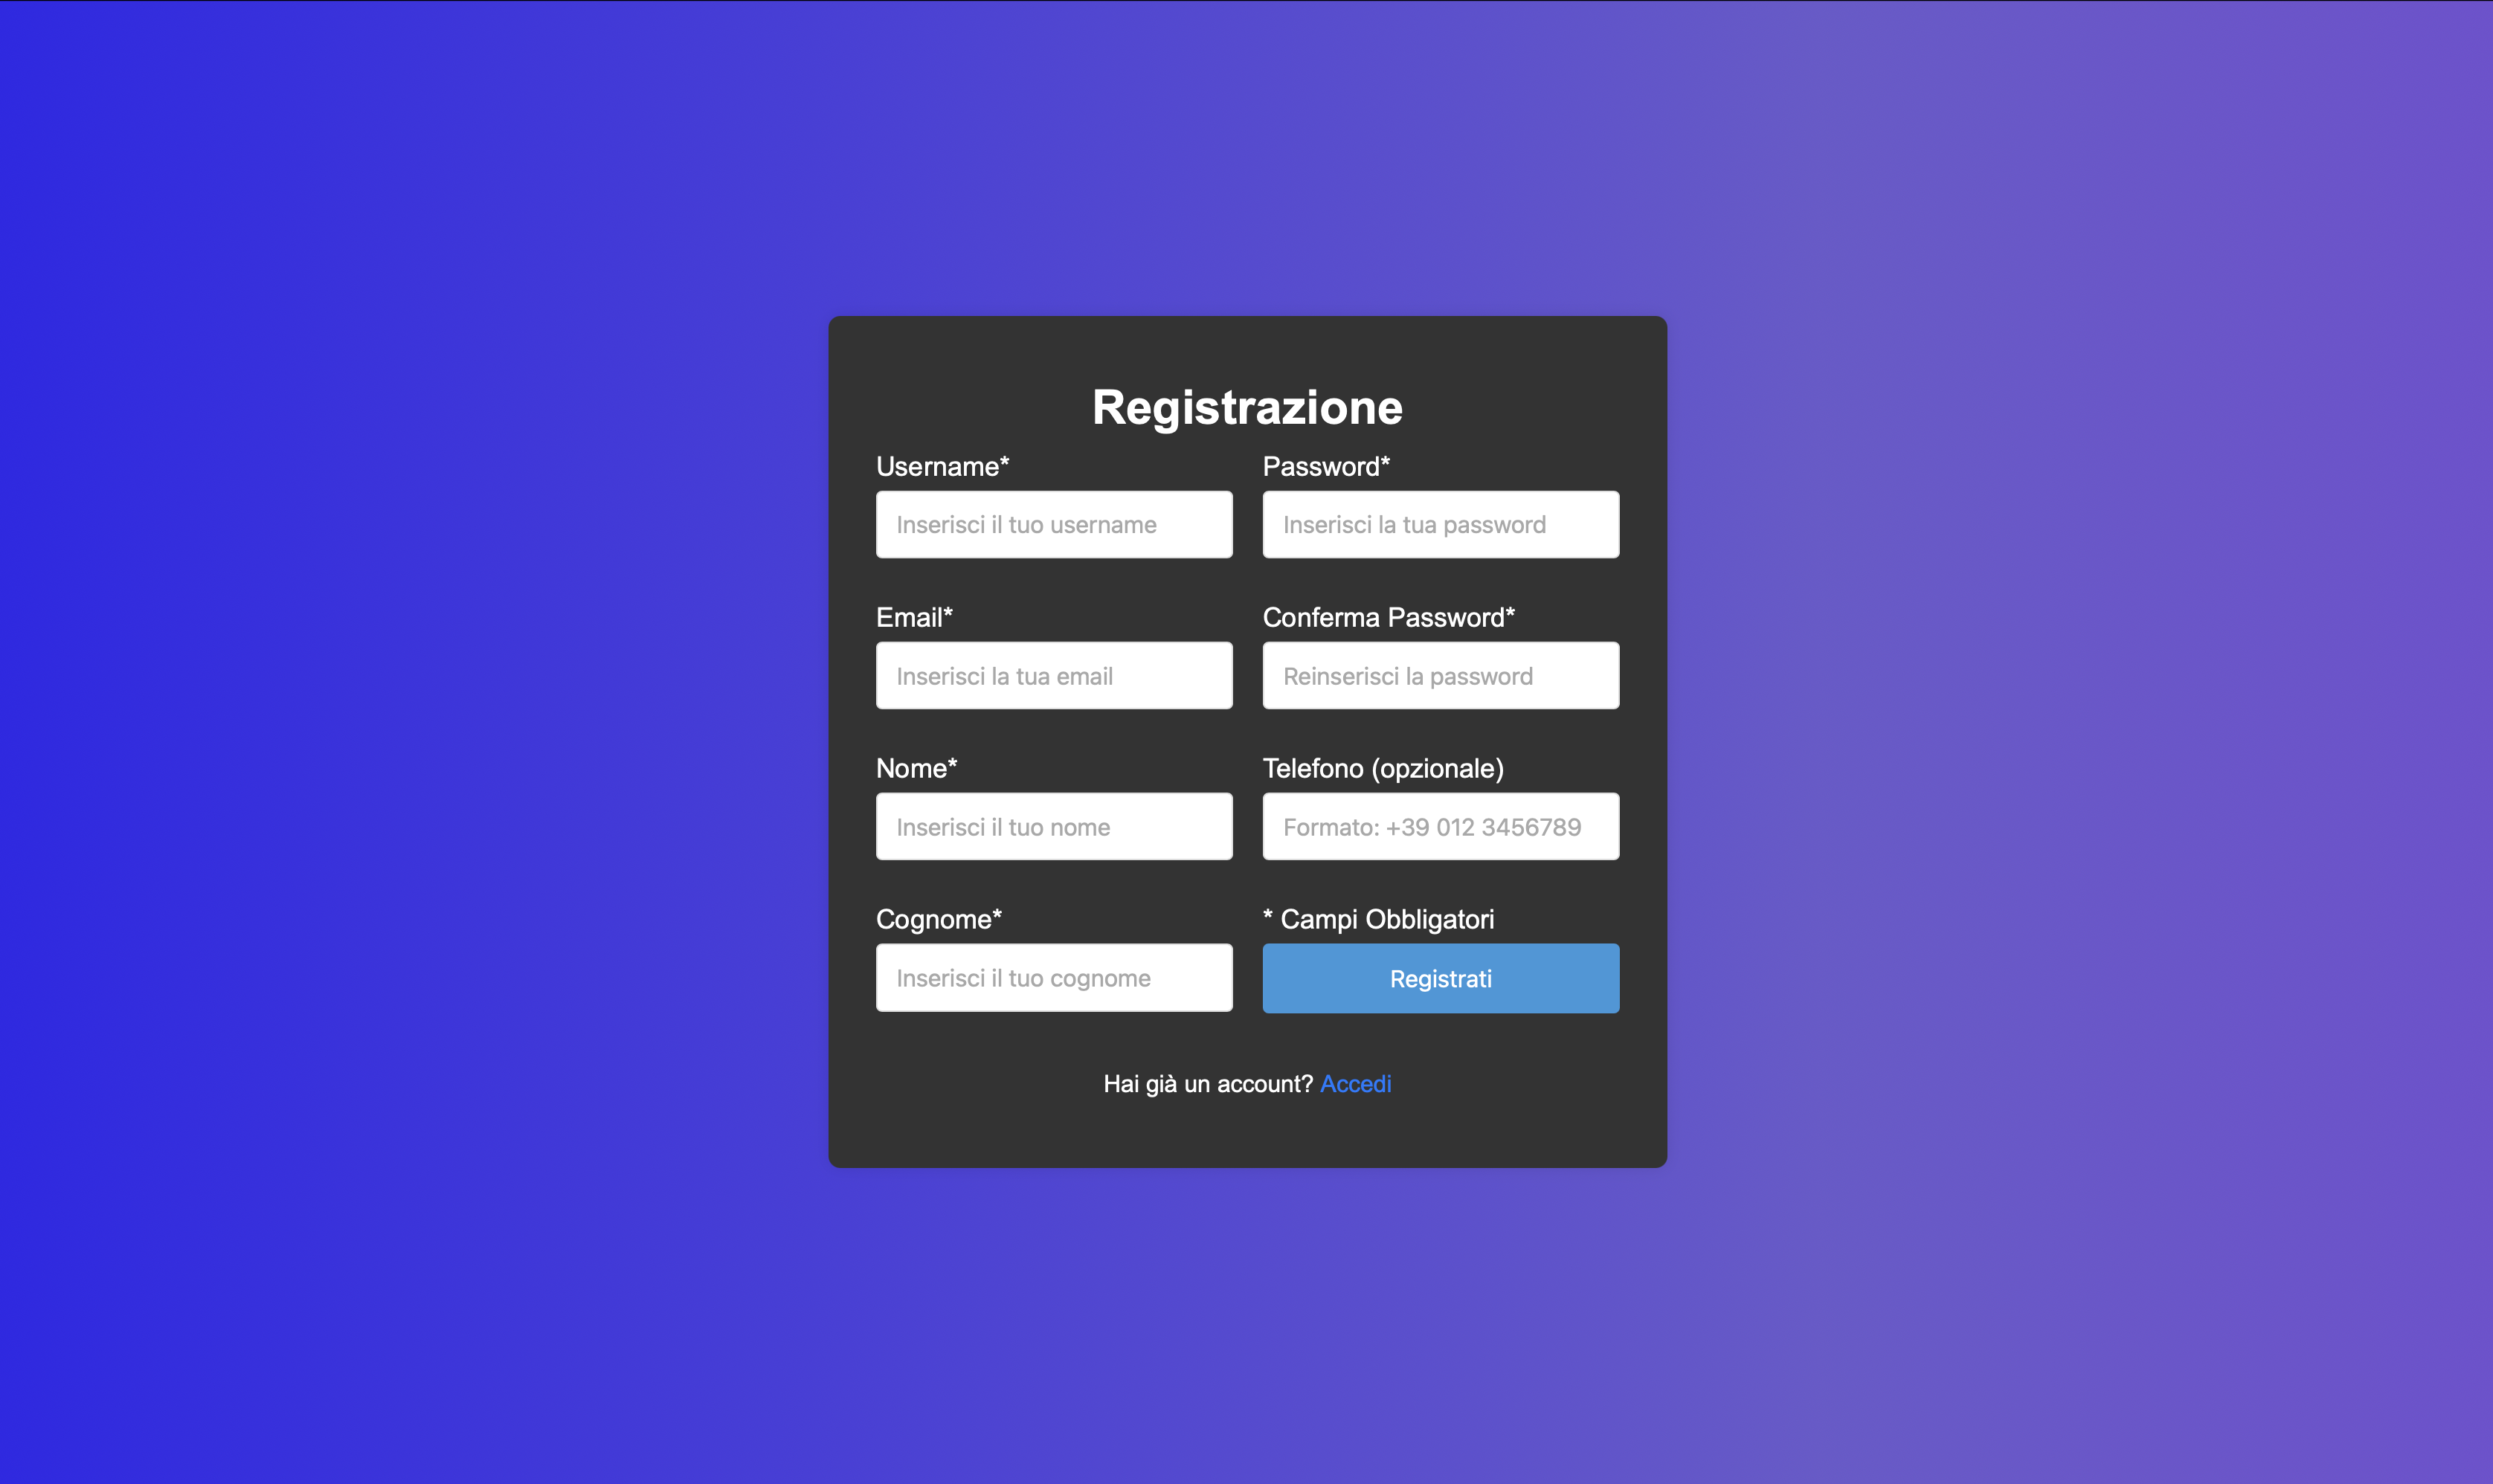
\includegraphics[width=0.8\textwidth]{./img/paginaRegistrazione.png}
    \caption{Schermata della pagina di registrazione}
\end{figure}

\subsection{Schermata iniziale}
Una volta effettuato l'accesso verremo accolti da questa Schermata iniziale composta da 3 elementi, una navbar superiore, una navbar laterale e il contenuto della pagina. Da qui è possibile iniziare una conversazione mettendo il titolo della conversazione e schiacciando il bottone: "inizia la conversazione".
\begin{figure}[h!]
    \centering
    \includegraphics[width=0.8\textwidth]{./img/paginaIniziale.png}
    \caption{Schermata della pagina di registrazione}
\end{figure}

\subsection{Schermata di conversazione}
Una volta creata la conversazione dalla schermata iniziale l'utente può andare nel menù laterale (\textit{nel caso esso sia chiuso si può aprire tramite menù ad hamburger}) e selezionare la voce: "\textit{Conversazioni salvate}" che aprirà un menù a tendina dove l'utente potrà selezionare la conversazione desiderata.
\begin{figure}[h!]
    \centering
    \begin{subfigure}{0.3\textwidth}
        \centering
        \includegraphics[width=\textwidth]{./img/laterale1.png}
    \end{subfigure}
    \hspace{0.05\textwidth}
    \begin{subfigure}{0.3\textwidth}
        \centering
        \includegraphics[width=\textwidth]{./img/laterale2.png}
    \end{subfigure}
    \caption{Menù laterale}
\end{figure}
L'utente si trovera quindi di fronte a una schermata composta da diversi elementi:
\begin{figure}[h!]
    \centering
    \includegraphics[width=\textwidth]{./img/SchermataChat1.png}
    \caption{Schermata della chat}
    \label{fig:schermata-chat}
\end{figure}
\\
Facendo riferimento alla figura~\ref{fig:schermata-chat} infatti l'utente troverà un bottone per selezionare una domanda templetizzata (\textit{qui segnato con il numero 1}), parleremo di queste più avanti.
Il punto numero 2 indica invece la casella di testo dove l'utente potrà scrivere il proprio messaggio da inviare al bot.
Il punto numero 3 indica il nome della conversazione precedentemente scelto nella schermata iniziale. Il punto numero 4 indica un bottone che permette di eliminare la chat premendolo apparirà un pop-up che chiede cortesemente all'utente se è sicuro di voler eliminare la conversazione figura~\ref{fig:elimina-chat}:
\begin{figure}[h!]
    \centering
    \includegraphics[width=0.5\textwidth]{./img/eliminaChat.png}
    \caption{Elimina chat}
    \label{fig:elimina-chat}
\end{figure}
\\
Il punto numero 5 in figura~\ref{fig:schermata-chat} è il pulsante invio che permette di mandare un messaggio al nostro assistente virtuale. Bisogna dire tuttavia che è possibile inviare un messaggio solo se del testo è presente nella casella di testo (\textit{punto 2 in figura~\ref{fig:schermata-chat}}) e che non è necessario cliccare sul pulsante in quanto è possibile premere direttamente invio sulla tastiera.
\\
Inviato un messaggio questo apparirà nella parte destra della schermata come avviene nelle più famose chat di messaggistica (fare riferimento a figura~\ref{fig:Elaborazione} punto 6), e verrà mostrato il messaggio e la data e l'ora dell'invio.
Nella parte sinistra l'utente potrà osservare il nostro Assistente virtuale Giorgione elaborare il messaggio per soddisfare la richiesta dell'utente (punto 7 figura~\ref{fig:Elaborazione}).
\begin{figure}[h!]
    \centering
    \includegraphics[width=\textwidth]{./img/SchermataChat2.png}
    \caption{Elaborazione del messaggio}
    \label{fig:Elaborazione}
\end{figure}
\\
Una volta mandato il messaggio esso sarà visualizzabile come mostrato in figura~\ref{fig:Visualizzazione Risposta} punto 8, e l'utente potrà decidere opzionalmente se è soddisfatto della risposta data dal bot di fornire una valutazione booleana indicata da un pollice in su e pollice in giù (\textit{figura~\ref{fig:Visualizzazione Risposta} punto 9}):
\begin{figure}[h!]
    \centering
    \includegraphics[width=\textwidth]{./img/SchermataChat3.png}
    \caption{Visualizzazione Risposta}
    \label{fig:Visualizzazione Risposta}
\end{figure}
L'utente è notificato dalla scelta dall'illuminazione di uno dei 2 bottoni come mostrato in figura~\ref{fig:likedislike}
\begin{figure}[h!]
    \centering
    \begin{subfigure}{0.2\textwidth}
        \centering
        \includegraphics[width=\textwidth]{./img/like.png}
        \caption{Caso in cui l'utente scelga like}
    \end{subfigure}
    \hspace{0.05\textwidth}
    \begin{subfigure}{0.2\textwidth}
        \centering
        \includegraphics[width=\textwidth]{./img/dislike.png}
        \caption{Caso in cui l'utente scelga dislike}
    \end{subfigure}
    \caption{Feedback Risposta}
    \label{fig:likedislike}
\end{figure}

\newpage

\section{Funzioni aggiuntive}

\subsection{Layout Responsive e Tema Scuro}
Il sito è stato ottimizzato per garantire un'esperienza utente fluida su dispositivi mobili tramite browser, grazie a un design completamente responsive. Ogni sezione del sito si adatta automaticamente alle dimensioni dello schermo, assicurando una visualizzazione ottimale. Inoltre, è stata implementata una funzionalità che consente agli utenti di alternare facilmente tra il tema chiaro e il tema scuro, offrendo una maggiore personalizzazione e comfort visivo.
\begin{figure}[h!]
    \centering
    \begin{subfigure}{0.3\textwidth}
        \centering
        \includegraphics[width=\textwidth]{./img/layoutResponsive1White.png}
    \end{subfigure}
    \hspace{0.05\textwidth}
    \begin{subfigure}{0.3\textwidth}
        \centering
        \includegraphics[width=\textwidth]{./img/layoutResponsive2White.png}
    \end{subfigure}
    \caption{Schermata pagina iniziale mobile tema chiaro}
\end{figure}

\begin{figure}[h!]
    \centering
    \begin{subfigure}{0.3\textwidth}
        \centering
        \includegraphics[width=\textwidth]{./img/layoutResponsive1Black.png}
    \end{subfigure}
    \hspace{0.05\textwidth}
    \begin{subfigure}{0.3\textwidth}
        \centering
        \includegraphics[width=\textwidth]{./img/layoutResponsive2Black.png}
    \end{subfigure}
    \caption{Schermata pagina iniziale mobile tema scuro}
\end{figure}

\newpage

\section{Supporto}
Per assistenza tecnica o domande relative all'utilizzo dell'assistente virtuale, è possibile contattare il supporto tecnico di \textit{Ergon Informatica} tramite la richiesta di supporto nella pagina dedicata o al nostro indirizzo mail:  
\begin{center}
    \href{mailto:code7crusaders@gmail.com}{code7crusaders@gmail.com}  
\end{center}
Per garantire un buon servizio che sia efficace e tempestivo, è importante fornire informazioni dettagliate sul problema riscontrato. Sarà nostro impegno rispondere in modo rapido e fornire assistenza per risolvere eventuali problemi o domande.

\end{document}
